\documentclass[12pt,a4paper]{article}

\usepackage[utf8]{inputenc}
\usepackage[margin=1in]{geometry}
\usepackage{graphicx}
\usepackage{amsmath,amssymb}
\usepackage{booktabs}
\usepackage{tabularx}
\usepackage{hyperref}
\usepackage{xcolor}
\usepackage{titlesec}
\usepackage{fancyhdr}
\usepackage{setspace}

\onehalfspacing

\hypersetup{
    colorlinks=true,
    linkcolor=blue!80!black,
    citecolor=blue!80!black,
    urlcolor=blue!80!black
}

\begin{document}

% =========================================================================
% PAGE 1: OFFICIAL VGU COVER PAGE (MATCHING TEMPLATE EXACTLY)
% =========================================================================
\begin{titlepage}
    \centering
    \vspace*{1.5cm}
    
    {\large Vietnamese-German University}\\[0.3cm]
    {\large Computer Science Study Program}\\[3.5cm]

    {\large 61CSE326 -- Project}\\[0.8cm]
    {\Large \textbf{Collaborative Stacker AMR for Warehouse-to-Aisle Stock Replenishment}}\\[3.5cm]

    {\large by}\\[0.8cm]
    {\large [Student Name 1, Matriculation No.]}\\
    {\large [Student Name 2, Matriculation No.]}\\
    {\large [Student Name 3, Matriculation No.]}\\
    {\large [Student Name 4, Matriculation No.]}\\[3.5cm]

    {\large Supervisor: Dr.-Ing. Quang Huan Dong}\\[2.5cm]

    \vfill
    {\large (September 15, 2026)}
\end{titlepage}

% =========================================================================
% PAGE 2: OFFICIAL DISCLAIMER PAGE (MATCHING TEMPLATE EXACTLY)
% =========================================================================
\newpage
\thispagestyle{plain}

\noindent \textbf{\Large Disclaimer}

\vspace{1.5cm}
\noindent We declare that this report is a product of our own work, unless otherwise referenced. We also declare that all opinions, results, conclusions, and recommendations are our own and may not represent the policies or opinions of the Computer Science study program of the Vietnamese-German University.

\vspace{4.5cm}
\noindent
\begin{tabularx}{\textwidth}{XX}
    \rule{5.5cm}{0.4pt} & \rule{5.5cm}{0.4pt} \\
    [Student Name 1] & [Student Name 2] \\[3cm]
    \rule{5.5cm}{0.4pt} & \rule{5.5cm}{0.4pt} \\
    [Student Name 3] & [Student Name 4] \\
\end{tabularx}

\newpage

% =========================================================================
% PAGE 3+: IMRaD STRUCTURE (WEEK 1 INITIAL SCOPING)
% =========================================================================
\pagestyle{fancy}
\fancyhf{}
\rhead{\small 61CSE326 -- Project Module}
\lhead{\small Collaborative Stacker AMR (UC6)}
\rfoot{\thepage}

\section{Introduction}

\subsection{Project Context \& Identification}
During autonomous warehouse and commercial facility operations, mobile transport robots frequently encounter obstacles such as misplaced storage pallets, structural pillars, and dynamic agents like walking personnel and manual carts. 

Under the module \textbf{61CSE326: Robot Obstacle-Avoidance Planning Software} at the Vietnamese-German University (VGU), supervised by Dr.-Ing. Quang Huan Dong, our team is investigating \textbf{Use Case 6 (UC6)}: \textit{A mobile robot navigates to storage locations, retrieves specified items from shelves, and transports them to designated drop-off points}.

\subsection{Official Repository Link}
The project source code, simulation assets, and documentation are hosted at:
\begin{center}
    \url{https://github.com/[Your-Org-Or-User]/61CSE326-Collaborative-Stacker-AMR}
\end{center}
\noindent
\textit{Note: The repository includes a \texttt{README.md} detailing environment setup. Read-only access has been granted to \texttt{huan.dq@vgu.edu.vn}.}

\subsection{Problem Statement \& Scope Formulation}
\paragraph{The Restocking Bottleneck:}
In commercial retail centers and fulfillment warehouses, transporting bulk stock from storage backrooms to retail display aisles constitutes over 50\% of manual labor hours, requiring workers to walk long routes pushing heavy carts.

\paragraph{Scope Definition (Warehouse-to-Aisle Logistics):}
Attempting fine-grained product placement directly onto customer-facing retail shelves requires complex manipulator arms, soft grippers, and costly 3D computer vision. To avoid this manipulation trap and keep our primary focus on the course's core objective---\textbf{obstacle avoidance}---we propose a \textbf{Collaborative Replenishment Workflow}:
\begin{enumerate}
    \item The Autonomous Mobile Robot (AMR) navigates to warehouse storage racks, lifts bulk totes/pallets, and ferries them to \textbf{Designated Staging Locations} (e.g., retail aisle endcaps).
    \item At these staging points, human staff unload the bulk stock and carry out the dexterous shelf-facing and stocking work.
\end{enumerate}

\paragraph{Core Problem Formulation:}
Operating across shared commercial corridors requires the path-planning software to handle:
\begin{enumerate}
    \item \textbf{Static Obstacle Avoidance:} Safely maneuvering around dropped packaging boxes, misplaced carts, and pillars.
    \item \textbf{Dynamic Obstacle Avoidance:} Detecting, slowing down, or replanning around moving pedestrians and crossing carts in shared aisles.
\end{enumerate}

\section{Methods \& Technical Investigation}

\subsection{System Architecture \& Simulation Pipeline (Under Evaluation)}
To establish a scalable digital twin environment, we are evaluating a hybrid architecture pairing \textbf{Unity (Unity 6 / 2022.3 LTS)} with \textbf{ROS 2 Humble Hawksbill}:
\begin{itemize}
    \item \textbf{Simulation Engine Testing (Unity):}
    \begin{itemize}
        \item Prototyping a 3D warehouse and retail corridor environment to model static spatial bounds.
        \item Testing Unity \texttt{ArticulationBody} components to assess realistic wheel traction and robot inertia.
        \item Evaluating simulated 2D planar LiDAR setups (360\circ$ raycasting) for publishing standard ROS 2 \texttt{sensor\_msgs/LaserScan} topics.
        \item Investigating Unity NavMesh agents for introducing controllable dynamic pedestrian clutter.
    \end{itemize}
    \item \textbf{Robotics Middleware Planning (ROS 2 Humble):}
    \begin{itemize}
        \item Analyzing \textbf{Navigation 2 (Nav2)} planners---specifically comparing ^*$/NavFn global planning against local reactive algorithms (Dynamic Window Approach - DWA, TEB Local Planner, and Artificial Potential Fields - APF).
        \item Assessing communication stability of the \texttt{ros\_tcp\_endpoint} bridge (port 10000).
    \end{itemize}
\end{itemize}

\subsection{Robot Structure \& Mechanism Concept}
Our proposed robot consists of two simple parts:
\begin{enumerate}
    \item \textbf{Two-Wheel Mobile Base:} The robot moves using two motorized wheels (differential drive) and small support caster wheels. This lets the robot turn in place smoothly on flat indoor floors.
    \item \textbf{Vertical Lift Mechanism:} Instead of a complex robotic arm with many moving joints, the robot uses a simple elevator-style lift (moving up and down by 10 to 30~cm). It raises to pick up a storage box and lowers to drop it off, controlled by a simple ROS 2 command (\texttt{/lift\_cmd}).
\end{enumerate}

\begin{figure}[htbp]
    \centering
    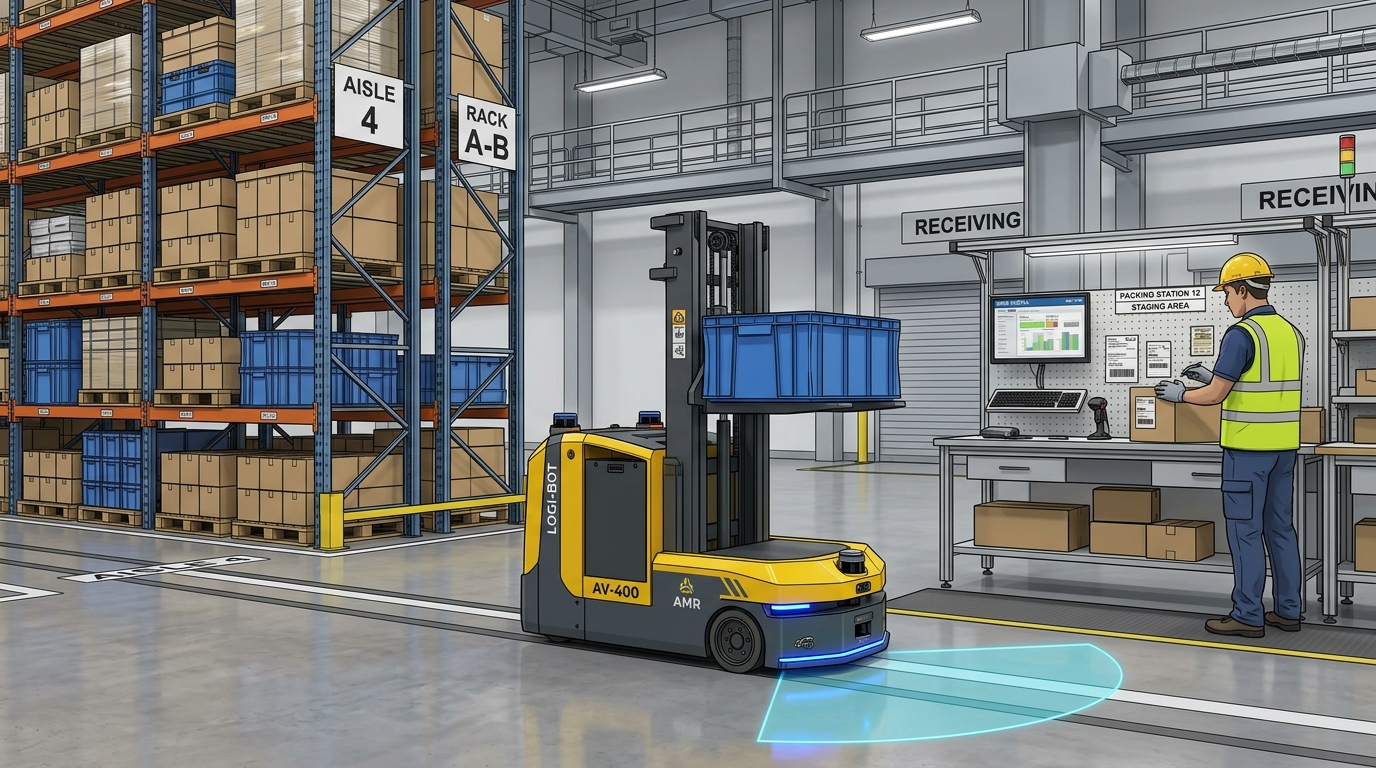
\includegraphics[width=0.82\linewidth]{warehouse_amr_concept.jpg}
    \caption{Conceptual rendering of the Collaborative Stacker AMR retrieving stock from warehouse storage and delivering to an aisle staging desk, showing planar 2D LiDAR coverage.}
    \label{fig:amr_concept}
\end{figure}

\subsection{Virtual-to-Hardware (Sim-to-Real) Abstraction Framework}
To ensure future physical hardware deployment remains feasible without rewriting our core logic (subject to timeline and resources):
\begin{itemize}
    \item Restricting core navigation interactions strictly to standard ROS 2 message definitions: \texttt{/cmd\_vel} (\texttt{geometry\_msgs/Twist}), \texttt{/scan} (\texttt{sensor\_msgs/LaserScan}), and \texttt{/odom} (\texttt{nav\_msgs/Odometry}).
    \item \textbf{Hardware Abstraction Planning:} Researching an embedded bridge path using \textbf{micro-ROS} on microcontrollers (\textbf{STM32 Nucleo} / \textbf{ESP32}) to replace the virtual Unity TCP socket when hardware prototyping begins.
\end{itemize}

\subsection{Team Organization \& Task Allocation}
The four team members are organized according to preliminary functional domains:
\begin{table}[htbp]
\centering
\small
\begin{tabularx}{\textwidth}{l p{3.5cm} X}
\toprule
\textbf{Role} & \textbf{Member} & \textbf{Primary Domain Responsibilities} \\
\midrule
\textbf{Team Lead / Systems} & [Student 1] & Git repository configuration, ROS 2 workspace architecture, coordinate frames (\texttt{tf2}), and micro-ROS hardware abstraction layer. \\
\textbf{Algorithm Engineer} & [Student 2] & ROS 2 Nav2 integration, Costmap2D parameter tuning, local reactive obstacle avoidance algorithms (DWA/TEB/APF). \\
\textbf{Simulation Engineer} & [Student 3] & Unity 3D environment setup, URDF robot importing, ArticulationBody physics tuning, and C\# LiDAR/motor communication scripts. \\
\textbf{Mission Logic \& QA} & [Student 4] & Weekly progress reporting, high-level Python mission coordinator state machine, test scenario design, and performance logging. \\
\bottomrule
\end{tabularx}
\caption{Team functional division of labor.}
\label{tab:roles}
\end{table}

\section{Results (Week 1 Progress)}
During the initial kickoff week, the following preliminary setup tasks were completed:
\begin{enumerate}
    \item \textbf{Scope \& Use Case Formulation:} Defined the Collaborative Warehouse-to-Aisle Stacker AMR use case, establishing clear boundaries between autonomous transport and human shelf stocking.
    \item \textbf{Development Environment Setup:}
    \begin{itemize}
        \item Configured native Ubuntu 22.04 LTS + ROS 2 Humble environments on team laptops.
        \item Configured an Ubuntu 24.04 LTS host with a dedicated Ubuntu 22.04 / ROS 2 Humble container via \textbf{Distrobox} on the Team Lead's laptop to maintain Linux Kernel 6.12 hardware driver stability.
        \item Installed Unity Hub, Unity 2022.3/6 LTS, and staged the \texttt{Unity-Robotics-Hub} packages.
    \end{itemize}
    \item \textbf{Project Governance:} Initialized the team GitHub repository, configured workspace directories, and prepared the weekly reporting structure.
\end{enumerate}

\section{Discussion}

\subsection{Environment Setup Findings \& Heterogeneous OS Strategy}
During our initial Week 0 setup, a major technical finding was the OS and hardware mismatch within the team:
\begin{itemize}
    \item While teammate laptops run native Ubuntu 22.04 LTS (Jammy) for direct compatibility with ROS 2 Humble, the Team Lead's modern Lenovo Yoga 7 requires Linux Kernel 6.12+ (Ubuntu 24.04 Noble) to support vendor-specific audio, Wi-Fi 6E, and touchscreen digitizers.
    \item Rather than risking hardware instability through an OS downgrade, we tested containerizing Ubuntu 22.04 and ROS 2 Humble using \textbf{Distrobox/Podman}. 
    \item \textbf{Outcome:} The container successfully shares the host \texttt{/dev} tree and network interfaces. This verifies that our team can maintain 100\% code compatibility on ROS 2 Humble without breaking laptop hardware support, while keeping direct USB serial access ready for future STM32/ESP32 hardware testing.
\end{itemize}

\subsection{Scope \& Design Feasibility (Lift vs. Arm)}
Our initial design discussions evaluated whether UC6 required a multi-axis robotic arm or a 1-DOF vertical lift:
\begin{itemize}
    \item Attempting individual item picking from retail shelves would demand inverse kinematics (MoveIt 2) and visual servoing. Given that 50\% of the course grade depends on Milestones 2 and 3 (Static and Dynamic Obstacle Avoidance), dedicating development hours to manipulator arm kinematics represents a severe timeline risk.
    \item Restricting the mechanism to a 1-DOF vertical lift transporting bulk totes to aisle endcaps satisfies the UC6 problem statement while leaving the vast majority of our timeline dedicated to costmaps, reactive avoidance, and dynamic obstacle handling.
\end{itemize}

\subsection{Week 1 Risks \& Technical Uncertainties}
As we transition into Week 1 tasks (establishing the ROS-TCP bridge and importing the URDF), our primary concerns are:
\begin{enumerate}
    \item \textbf{Unity 6 / 2022 LTS Package Compatibility:} Verifying whether \texttt{ROS-TCP-Connector} and URDF Importer compile cleanly in our Unity environment without deprecated API conflicts.
    \item \textbf{Bridge Latency:} Measuring the round-trip latency over the TCP socket (port 10000) when streaming simulated 360$^\circ$ LiDAR scans to ensure it does not bottleneck real-time local path planning.
\end{enumerate}

\end{document}
